% COMS E6998-007 final report, first draft (2026-11-07); 9B serving follow-up added 2026-11-10.
% 2026-11-10: Table 2 marks its eight unmeasured LLM cells (NM) and cell status; tab:allrouting lists every routing policy.
% Build: see paper/README.md. Numbers trace to reports/ and records/ (Appendix C).
\documentclass[11pt]{article}

\usepackage{acl}
\usepackage{times}
\usepackage{latexsym}
\usepackage[T1]{fontenc}
\usepackage[utf8]{inputenc}
\usepackage{microtype}
\IfFileExists{inconsolata.sty}{\usepackage{inconsolata}}{\renewcommand{\ttdefault}{lmtt}}
\usepackage{graphicx}
\usepackage{booktabs}
\usepackage{amsmath}
\usepackage{amssymb}
\usepackage{xcolor}
\usepackage{tikz}
\usetikzlibrary{positioning,arrows.meta}

\newcommand{\pp}{\,pp}
% Let the two full-width serving figures share a page.
\renewcommand{\dbltopfraction}{0.85}

\title{When Can Open Decision Models Replace Generative LLM Calls?}

\author{Ju Zhang \\
  Columbia University \\
  \texttt{jz3702@columbia.edu} \\\And
  Weiyu Chen \\
  Columbia University \\
  \texttt{wc2973@columbia.edu} \\\And
  Yizhi Hu \\
  Columbia University \\
  \texttt{yh4060@columbia.edu}}

\begin{document}
\maketitle

\begin{abstract}
Many production LLM calls make classification-shaped decisions such as intent routing and evidence checks. We study when open decision models, which score a fixed label set in one forward pass and return a probability distribution, can replace these calls, and when deferring uncertain inputs to a generative LLM pays off. Across CLINC150 banking intents with out-of-scope queries, SQuAD~2.0 answerability and ANLI, the StartLux-4B decision model is 5.3--18.8 points more accurate than the same-size Qwen3.5-4B generative LLM and sustains 1.8--1.9$\times$ its throughput at concurrency 8 on one L40S GPU. Deferring to the generative model added little. A confidence-gated cascade on SQuAD gained 0.25 points (95\% CI $-0.29$ to $0.83$), a gain-aware router trailed confidence routing on a fresh 4,000-question holdout ($-0.225$ points, CI $-0.91$ to $0.48$), and on ANLI the router fitted on validation chose never to defer, even though a 9B fallback could have corrected 289 front-model errors (it would also have broken 544 correct answers). Validation-selected operating points did not transfer. The 5\% selective-risk target was missed for three of four front-model/task pairs, and a 10\% deferral budget became 23\% on ANLI. Under open-loop load with a 500\,ms SLO, a CPU classifier built on a frozen MiniLM encoder and trained on 1,600 labels lands 0.33 points below the decision model on CLINC and stays on time at 100 requests/s, a load at which both GPU services saturated under our serving settings. In a retrospective size control, scaling the decision model from 4B to 9B adds 2.5 points on ANLI (95\% CI 1.3--3.8), more than any of the frozen cascades we evaluated with a 9B generative fallback. A follow-up served both options on one GPU. At each tested load from 10 to 80 requests/s, the 9B decision model returned more correct answers within 500\,ms than the most accurate frozen 4B-to-9B cascade, with 0.50 of GPU memory against the cascade's 0.90, and at 80 requests/s the 4B model alone returned the most.
\end{abstract}

\section{Introduction}

Many LLM calls in deployed systems choose among a fixed set of options. A banking assistant routes a request to one of fifteen intents or rejects it as out of scope; a retrieval pipeline checks whether a passage answers a question. A generative LLM prompted to return only the label, as in our constrained-JSON setup, spends a decoding pass on every decision and reports no distribution over the options. Decision models score a fixed set of candidate labels in one forward pass and return a distribution over them \citep{li2026jevcascade,zhuang2026startlux}. That distribution suggests a cascade, in which the decision model answers when it is confident and defers the remaining inputs to a generative model, as cost-aware LLM cascades do for open-ended generation \citep{chen2023frugalgpt,gupta2024cascades}.

We evaluate this design with released checkpoints and real serving measurements, around three research questions.

\textbf{RQ1} How accurately do frozen decision models make these decisions directly, compared with a same-size generative LLM and with cheap supervised classifiers?

\textbf{RQ2} When does deferring low-confidence inputs to the generative model improve on the best direct system, and do operating points selected on validation data hold on new test data?

\textbf{RQ3} How do serving constraints (throughput, latency SLOs, co-residency) change which deployment is best?

We study CLINC150 banking intents with out-of-scope (OOS) queries \citep{larson-etal-2019-evaluation}, SQuAD~2.0 answerability \citep{rajpurkar-etal-2018-know} and ANLI \citep{nie-etal-2020-adversarial}, using Kev-4B \citep{kev4b}, StartLux-Decision 4B and 9B \citep{zhuang2026startlux} and Qwen3.5 4B and 9B \citep{qwen35}. All weights stay frozen. Every threshold and routing policy is fitted on calibration and validation data and frozen before test predictions are scored, and the gold labels of the two main holdouts stayed sealed until evaluation. Across three studies and four follow-ups we collected 47,650 LLM predictions, 7,400 CPU classifier predictions and about 720,000 timed serving requests in single-GPU NVIDIA L40S allocations; serving requests repeat inputs that were already scored and are counted apart from predictions.

Our findings are as follows.
\begin{itemize}
\item Among the 4B models evaluated on each task, StartLux-4B is the most accurate, ahead of Qwen3.5-4B by 5.3 to 18.8 points, and it serves 1.8--1.9$\times$ as many requests per second. Kev-4B was evaluated on CLINC and the Study~1 SQuAD test only.
\item In our studies, deferral to the generative model produced no confirmed improvement over direct StartLux. A gain-aware router trails confidence routing on a fresh holdout, and on ANLI the router fitted on validation defers nothing. Complementary errors exist in hindsight, but the features available at routing time do not identify them.
\item Operating points chosen on validation drift on test, in both directions. A 10\% budget becomes 23\% for confidence routing and 0.6\% for a gain router on ANLI.
\item Under open-loop load, a frozen MiniLM encoder with a logistic head comes within 0.33 points of StartLux on CLINC and answers every request on time at 100 requests/s with one inference thread (about 0.5 CPU core-equivalents on average), while under our client and vLLM settings the GPU services saturate near 65 (StartLux) and 47 (Qwen) completions per second.
\item On ANLI, the 9B decision model (76.69\%) is more accurate than each frozen cascade we evaluated that adds a 9B generative fallback to the 4B model (at most 74.41\%). Served under open-loop load, it also returned more correct answers within 500\,ms than the most accurate of these cascades at every tested rate, and at the highest load the 4B model alone returned the most correct answers on time.
\end{itemize}
We release the evaluation harness, frozen protocols, audit scripts and a CPU-only Decision Lab that replays recorded cases and the measured follow-ups (Appendix~C).

\section{Related Work}

\paragraph{Cascades and routing.}
Two families of methods decide when to spend a larger model. Cascades call the small model first and escalate after seeing its output. FrugalGPT chains LLM APIs of increasing cost and stops when a learned scorer accepts the answer \citep{chen2023frugalgpt}, AutoMix escalates based on the small model's self-verification \citep{aggarwal2024automix}, and \citet{gupta2024cascades} show that naive sequence-level uncertainty is a weak deferral signal for generative cascades and learn deferral rules from token-level features. Routers choose a model before any generation, from the query alone. RouteLLM learns that choice from preference data \citep{ong2024routellm}, and Hybrid LLM from the predicted quality gap between a small and a large model \citep{ding2024hybrid}. Our cascades belong to the first family, with a decision model as the front model. Its single forward pass returns a full label distribution, so the routing signal costs one prefill pass, and every task has an exact label, so we can count rescued and harmed inputs for each policy and compare against matched-quota random and oracle routing. JevCascade studies inference-time compute allocation within prefill-only decision models and shows that accuracy after changing the candidate menu can be predicted from cached first-pass probabilities \citep{li2026jevcascade}. We study deferral to a separate generative model and its serving cost.

\paragraph{Selective prediction and risk control.}
Accepting a prediction only when confidence clears a threshold is the reject option of \citet{chow1970optimum}. Selective classification makes the risk--coverage trade-off explicit and gives a high-probability risk bound for a chosen threshold \citep{geifman2017selective}, and Learn then Test provides finite-sample risk control through multiple testing \citep{angelopoulos2021ltt}. Our gate is the empirical version used in practice, maximum coverage subject to at most 5\% validation error, and we measure how often that target holds on new data.

\paragraph{Calibration and prevalence shift.}
Temperature scaling fixes much of the miscalibration of modern networks with a single parameter \citep{guo2017calibration}. Changes in class prevalence move both posterior probabilities and the error rate of a fixed threshold \citep{saerens2002adjusting,lipton2018detecting}, and \citet{iqbal2026typed} examine how decision models' calibration and thresholds behave as class frequencies change between development and deployment. Our CLINC stress workload raises the OOS share from 25\% to 65\%, and the ANLI holdout shifts the confidence distribution between train-derived validation data and the official test.

\paragraph{Encoder classifiers.}
Sentence encoders such as Sentence-BERT and MiniLM give strong text representations at a small fraction of an LLM's cost \citep{reimers-gurevych-2019-sentence,wang2020minilm}, and SetFit shows that a few labelled examples per class suffice for competitive classification \citep{tunstall2022setfit}. We include TF-IDF and frozen MiniLM with logistic heads to test whether a 4B model is needed at all.

\paragraph{LLM serving.}
vLLM's PagedAttention made high-throughput batched serving practical \citep{kwon2023vllm}, and DistServe argues for SLO goodput, the rate of requests completed within their latency targets, as the serving objective \citep{zhong2024distserve}. We report SLO goodput and add a correctness requirement.

\section{Tasks, Data and Models}

\begin{table*}[t]
\centering
\small
\begin{tabular}{lcrrp{0.36\textwidth}l}
\toprule
Task & Labels & Calib. & Valid. & Test / holdout & Bootstrap unit \\
\midrule
CLINC banking + OOS & 16 & 400 & 400 & 600 main (450 banking, 150 OOS); 850 extra OOS for the stress workload & class strata \\
SQuAD~2.0 answerability & 2 & 1,000 & 1,000 & Study 1: 2,000 from 35 dev articles & article \\
 & & & & Study 2: 4,000 from 57 unused train articles (sealed) & article \\
ANLI R1--R3 & 3 & 1,800 & 900 & 3,200 official test, R1/R2/R3 = 1,000/1,000/1,200 (sealed) & premise (2,854) \\
\bottomrule
\end{tabular}
\caption{Evaluation data. Calibration fits temperatures and router heads; validation selects thresholds; test and holdout sets are scored once after freezing. SQuAD and ANLI test sets are class-balanced.}
\label{tab:data}
\end{table*}

\paragraph{Tasks.}
Table~\ref{tab:data} summarises the splits. CLINC uses the fifteen banking intents of CLINC150 plus the OOS label \citep{larson-etal-2019-evaluation}. The stress workload reuses the 450 banking test inputs and adds the remaining 850 OOS test inputs, raising the OOS share from 25\% to 65.4\%. SQuAD~2.0 is reduced to given-passage answerability (answerable or unanswerable) and is scored by accuracy. Calibration and validation come from article-disjoint subsets of the training set, the Study~1 test set from the official dev set, and the Study~2 holdout from 57 training articles that no earlier split used. ANLI keeps all 3,200 official test items; calibration and validation come from the training set after removing every premise that also appears in test, and the input carries only premise, hypothesis and label definitions. All splits are selected by hashing sample IDs with a fixed seed, sources are pinned by SHA-256, and duplicates with conflicting labels are dropped.

\paragraph{Models.}
The decision models are Kev-4B v1.0, an adapter and decision head on Qwen3.5-4B-Base \citep{kev4b}, and StartLux-Decision-v1.1 4B and 9B Instant \citep{zhuang2026startlux}, read through their native label-scoring interfaces, with StartLux's deliberation mode disabled. The generative models are Qwen3.5-4B and Qwen3.5-9B \citep{qwen35}, prompted with the same task instruction and label definitions, with thinking disabled, temperature 0 and a JSON output constrained to the label set; they return a label without probabilities. StartLux and Qwen run in vLLM 0.31.0 in BF16 with an 8,192-token limit, no truncation and prefix caching disabled; Kev runs on its official PyTorch serving stack. Revisions are pinned (Appendix~C).

The CPU baselines are TF-IDF over word unigrams and bigrams and a frozen all-MiniLM-L6-v2 encoder (ONNX, mean pooling, 384 dimensions) \citep{wang2020minilm,reimers-gurevych-2019-sentence}, each followed by an L2-regularised logistic regression ($C{=}1$). They are trained on either the 400 CLINC calibration examples or a 1,600-example pool of 1,500 banking and 100 OOS training examples.

\paragraph{Exposure.}
All three datasets are public, so pretraining exposure is unknown for every model. CLINC150 was part of StartLux's development panel and of a Kev temperature comparison. Our results therefore describe released systems on these tasks; separating architecture from training data would require controlled checkpoints.

\section{Methods}

\begin{figure}[t]
\centering
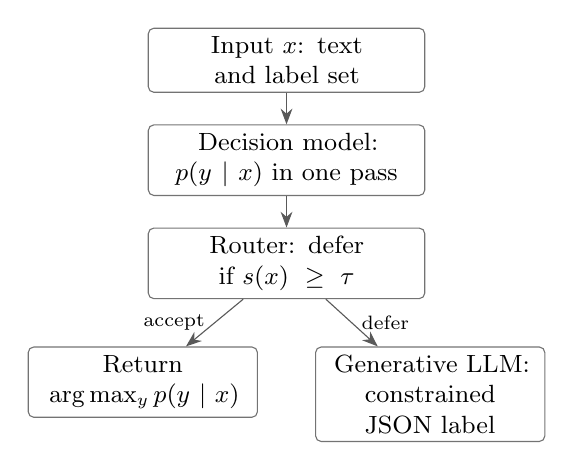
\begin{tikzpicture}[font=\small, node distance=4mm and 6mm,
  box/.style={draw=black!55, rounded corners=2pt, align=center, inner sep=3pt, minimum height=8mm, text width=33mm},
  arr/.style={-{Stealth[length=2mm]}, draw=black!65}]
\node[box] (x) {Input $x$: text and label set};
\node[box, below=of x] (dm) {Decision model:\\ $p(y\mid x)$ in one pass};
\node[box, below=of dm] (r) {Router: defer if $s(x)\ge\tau$};
\node[box, below left=6mm and -14mm of r, text width=27mm] (acc) {Return $\arg\max_y p(y\mid x)$};
\node[box, below right=6mm and -14mm of r, text width=27mm] (gen) {Generative LLM:\\ constrained JSON label};
\draw[arr] (x) -- (dm);
\draw[arr] (dm) -- (r);
\draw[arr] (r) -- node[left, font=\scriptsize] {accept} (acc);
\draw[arr] (r) -- node[right, font=\scriptsize] {defer} (gen);
\end{tikzpicture}
\caption{The cascade. Router scores $s(x)$ are defined in \S\ref{sec:routers}; $\tau$ is frozen on validation data.}
\label{fig:system}
\end{figure}

\paragraph{Recalibration.}
For Kev and StartLux we compare released probabilities with a task-specific temperature $T$ fitted on calibration data, $p_T(y\mid x)\propto\exp(\log p(y\mid x)/T)$ \citep{guo2017calibration}, and report NLL, Brier score and ECE with 15 equal-width bins.

\paragraph{Selective acceptance (primary endpoint).}
The gate accepts the decision model's label when $\max_y p(y\mid x)\ge\tau$. On validation data, $\tau$ maximises coverage subject to at most 5\% error among accepted inputs and at least 50 accepted inputs; tied scores are accepted or rejected together. The primary endpoint of Study~1 is test coverage together with test selective risk (error among accepted inputs) at the frozen $\tau$, with 95\% intervals. We report misses of the 5\% target and make no risk guarantee.

\paragraph{Cascades and matched-quota controls.}
Rejected inputs take the generative model's actual prediction (Figure~\ref{fig:system}). A deferral \emph{rescues} an input when the front model is wrong and the fallback right, and \emph{harms} it in the opposite case. At the same number of deferrals $k$ we compare against random routing (analytic expectation) and a hindsight oracle that defers the $k$ inputs with the largest gain $\delta_i = \mathbf{1}[\text{fallback correct}]-\mathbf{1}[\text{front correct}]$. The oracle uses gold labels and is an upper bound.

\paragraph{Routers.}
\label{sec:routers}
Studies 2 and 3 compare routers that defer when a score $s(x)$ reaches a threshold frozen on validation, with a deferral budget of 10\% of validation inputs (Study~2 also reports 5\% and 20\%). \emph{Confidence} uses $s=1-\max_y p(y\mid x)$. \emph{Class-conditional} fits a logistic model of front-model correctness on the logit of the maximum probability and the predicted class, with $s=1-\hat P(\text{front correct})$. \emph{Gain} fits separate correctness models for the front and the fallback, adding $\log(1+\text{input length})$, and uses $s=\hat P(\text{fallback correct})-\hat P(\text{front correct})$. \emph{Fixed gain} fills the budget with the highest gain scores; \emph{positive gain} (Study~3) admits only inputs with $s>0$ and may defer nothing. The heads use L2 penalty 0.01 with features standardised on calibration data. In Study~2 the validation set chose between class-conditional and gain as the primary candidate; Study~3 fixed positive gain with the Qwen3.5-9B fallback as primary before any prediction.

\paragraph{Statistics.}
Intervals are paired percentile bootstraps with 2,000 replicates and seed 6998, resampling SQuAD articles, ANLI normalised premises and CLINC within class strata \citep{field2007bootstrapping}. Each study has one prespecified primary comparison; everything else is descriptive and uncorrected for multiplicity. Intervals condition on the frozen models, prompts and thresholds.

\paragraph{Protocol and audit.}
Data manifests, configurations and source files are hash-pinned. Policies are frozen before holdout predictions, holdout gold is sealed with a first-access receipt, and every accepted final result bundle is archived by SHA-256 and re-scored by an independent script that does not import project code.

\paragraph{Serving measurements.}
\emph{Closed loop} (Study~1): five deployments (Kev, StartLux and Qwen alone; Kev$\to$Qwen and StartLux$\to$Qwen cascades) process fixed 200-input workloads per task at client concurrency 1 and 8 for three rounds of at least 30\,s; throughput is inputs per wall-clock second and latency runs from worker start. \emph{Open loop}: requests arrive as a Poisson process at a fixed offered rate, all conditions share the same arrival schedule, each request gets one HTTP attempt, and the client holds at most 64 active or queued requests. The SLO is 500\,ms from scheduled arrival to completion, so it includes client queueing. SLO goodput counts on-time successful responses per second of offered window, and correct goodput also requires the correct label. Study~2 compares StartLux alone, StartLux and Qwen co-resident with Qwen idle, the frozen gain cascade and Qwen alone at 10, 25 and 40 requests/s (3 rounds of 30\,s, 8 workers). The service study compares MiniLM-400 and MiniLM-1600 on one CPU thread with batch size 1 against StartLux-4B and Qwen3.5-4B (GPU memory share 0.4) at 5, 25 and 100 requests/s (5 rounds of 180\,s, 16 workers), restarting and warming up each service before every cell. The 9B serving follow-up compares StartLux-4B, StartLux-9B and a cascade from StartLux-4B to Qwen3.5-9B with both engines resident, on the 3,200 ANLI test inputs at 10, 20, 40 and 80 requests/s (3 rounds of 120\,s, 16 workers), with the same restart and warm-up before every cell. Its cascade uses the class-conditional router, the most accurate frozen Study~3 cascade offline; it was picked after Study~3 and kept fixed. The memory share is vLLM's GPU memory utilisation per engine. Studies~1--2 and the service study used 0.40 per model, also when two models were resident; Study~3 and the size control collected 9B predictions one model at a time with a 0.80 share and measured quality only. A 0.40 share (17.8\,GiB of the 44.4\,GiB visible to vLLM) cannot hold the 16.8\,GiB of 9B weights together with activations and a KV cache, so both 9B models ran at 0.50, which puts the cascade at 0.90; every engine in this follow-up was capped at 64 concurrent sequences. It adds a 1,000\,ms SLO and counts a tested rate as sustained only when every round answered at least 99\% of offers on time. Each study ran in a single-GPU Slurm allocation with one NVIDIA L40S (46\,GB), 100\,GB host RAM and AMD EPYC 7643 cores; allocations and physical cards differ between studies.

\section{Results}

\subsection{RQ1: Direct decisions}

\begin{table}[t]
\centering
\small
\setlength{\tabcolsep}{3pt}
\resizebox{\columnwidth}{!}{%
\begin{tabular}{lrrrr}
\toprule
 & CLINC & \multicolumn{2}{c}{SQuAD~2.0} & ANLI \\
\cmidrule(lr){3-4}
Model & main & S1 test & S2 holdout & test \\
\midrule
Kev-4B & 77.50 & 81.35 & NM & NM\phantom{$^\dagger$} \\
StartLux-4B & 93.50 & 91.25 & 91.78 & 74.19\phantom{$^\dagger$} \\
StartLux-9B & NM & NM & NM & 76.69\smash{$^\dagger$} \\
Qwen3.5-4B & 88.00 & 86.00 & 85.95 & 55.41\phantom{$^\dagger$} \\
Qwen3.5-9B & NM & NM & NM & 66.22\phantom{$^\dagger$} \\
\midrule
\multicolumn{5}{l}{\emph{CPU classifiers, CLINC-only protocol}\smash{$^\dagger$}} \\
TF-IDF + LR (400) & 73.83 & -- & -- & -- \\
TF-IDF + LR (1,600) & 84.50 & -- & -- & -- \\
MiniLM + LR (400) & 90.67 & -- & -- & -- \\
MiniLM + LR (1,600) & 93.17 & -- & -- & -- \\
\bottomrule
\end{tabular}
}
\caption{Direct accuracy (\%) on the CLINC main test ($n{=}600$), two SQuAD~2.0 answerability splits and the ANLI official test ($n{=}3{,}200$). S1 is the Study~1 test set (2,000 questions from official dev articles) and S2 the Study~2 holdout (4,000 questions from unused training articles). NM: not measured; no prediction exists for these eight LLM cells. --: outside the CPU baseline protocol, which trained and evaluated these classifiers on CLINC only, so no SQuAD or ANLI prediction was attempted. Cells differ in status, and none is a primary endpoint. Unmarked cells are descriptive results of the study that owns the column (Study~1 for CLINC and S1, Study~2 for S2, Study~3 for ANLI), scored once after that study's freeze. $^\dagger$Retrospective, collected after an earlier study had scored the same test set: the StartLux-9B cell is a size control, and the CPU rows are trained on the stated number of CLINC labels.}
\label{tab:direct}
\end{table}

Among the 4B models evaluated on each task, StartLux-4B is the most accurate (Table~\ref{tab:direct}); Kev-4B has no S2 or ANLI measurement, so on those two sets the comparison covers StartLux-4B and Qwen3.5-4B only. StartLux-4B's paired advantage over Qwen3.5-4B is 5.50 points on CLINC (95\% CI 3.67--7.33) and 5.25 on the S1 SQuAD test (3.59--6.82), and it reaches 5.83 on the fresh S2 holdout and 18.78 on ANLI. On CLINC all three LLMs recall 148 of 150 OOS queries, so the gap comes from the banking intents, where accuracy is 70.44\% for Kev, 84.44\% for Qwen and 91.78\% for StartLux. Qwen3.5-9B gains 10.8 points over its 4B sibling on ANLI and remains 7.97 points below StartLux-4B.

The supervised CPU classifiers close most of the gap on CLINC. MiniLM-1600 answers 559 of 600 main-test inputs correctly against StartLux's 561, with a different error profile. It is more accurate on banking intents (95.11\% vs.\ 91.78\%) and recalls fewer OOS queries (87.33\% vs.\ 98.67\%). MiniLM is correct on 26 inputs StartLux misses, and StartLux on 28 that MiniLM misses. More labels did not help uniformly. Moving MiniLM from 400 to 1,600 labels raised main-test accuracy by 2.50 points and lowered accuracy on the OOS-heavy stress workload by 3.15 points; the larger pool also lowers the OOS share of training data from 25\% to 6.25\%, so the two effects are confounded.

StartLux-9B improves on StartLux-4B by 2.50 points on ANLI (95\% CI 1.34--3.81), with gains in all three rounds (R1 84.9 vs.\ 82.6, R2 75.2 vs.\ 72.7, R3 71.1 vs.\ 68.4). It is correct on 245 items the 4B model misses and wrong on 165 the 4B model gets right.

\subsection{Selective acceptance}

\begin{table}[t]
\centering
\small
\setlength{\tabcolsep}{3pt}
\resizebox{\columnwidth}{!}{%
\begin{tabular}{llrrr}
\toprule
Task & Front & Coverage [95\% CI] & Selective risk [95\% CI] & Defer \\
\midrule
CLINC & Kev (rel.) & 65.00 [62.17, 67.83] & 6.67 [4.58, 8.79] & 210 \\
CLINC & Kev (refit) & 64.17 [61.17, 67.00] & 7.53 [5.29, 9.70] & 215 \\
CLINC & StartLux & 99.83 [99.50, 100.00] & 6.34 [4.67, 8.18] & 1 \\
SQuAD & Kev & 35.40 [31.72, 39.08] & 4.38 [2.57, 6.67] & 1,292 \\
SQuAD & StartLux & 93.75 [92.35, 94.93] & 6.29 [4.54, 8.51] & 125 \\
\bottomrule
\end{tabular}
}
\caption{Primary endpoint of Study~1: test coverage (\%) and selective risk (\% error among accepted inputs) at thresholds frozen on validation with a 5\% target, with 95\% paired percentile bootstrap intervals (CLINC resampled within class strata, SQuAD by article). Released (rel.) and refitted temperatures give identical gates except for Kev on CLINC.}
\label{tab:risk}
\end{table}

The validation target did not carry over to test (Table~\ref{tab:risk}). Selective risk exceeds 5\% for three of the four front-model/task pairs, and the interval for refitted Kev on CLINC excludes 5\%. StartLux accepted all 400 CLINC validation inputs with five errors (1.25\%) and then made 38 errors among 599 accepted test inputs. Kev's SQuAD gate met the target in point estimate at 35\% coverage, with an interval reaching 6.67\%. Prevalence also moves the measured risk. On the stress workload, where OOS queries are 65\% of inputs, selective risk falls to 3.31\% for StartLux and 2.51\% for Kev with the same banking predictions, because the added OOS inputs are easy.

Temperature refitting changed probability quality in mixed directions (Appendix Table~\ref{tab:prob}). It improved NLL, Brier score and ECE for Kev on SQuAD and slightly reduced ECE while raising NLL and Brier score on CLINC. On binary SQuAD a temperature is a monotone transform of the confidence score, so the accepted sets did not change.

\subsection{RQ2: Deferral to a generative model}

\begin{figure}[t]
\centering
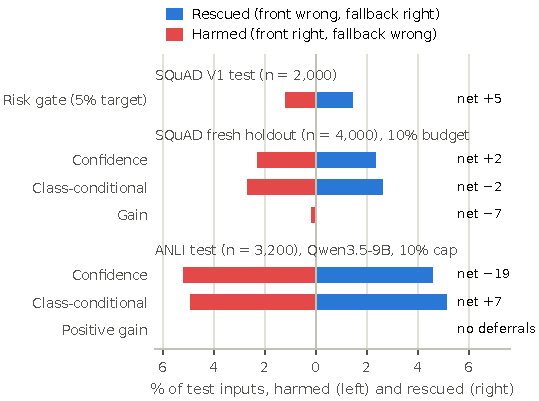
\includegraphics[width=\columnwidth]{figures/fig_rescue_harm.pdf}
\caption{Rescued and harmed inputs per deferral policy, as a share of each test set, with net change in correct answers. All policies use StartLux-4B as the front model and thresholds frozen on validation. Rows show the Study~1 SQuAD gate, Study~2 at its 10\% budget and Study~3 with the Qwen3.5-9B fallback (its fixed-gain policy, with no rescue or harm, is left out); Appendix Table~\ref{tab:allrouting} lists every policy.}
\label{fig:rescue}
\end{figure}

\begin{table}[t]
\centering
\small
\setlength{\tabcolsep}{3pt}
\resizebox{\columnwidth}{!}{%
\begin{tabular}{lrrr}
\toprule
Policy & Acc. & Defer \% (val$\to$test) & Resc./harm \\
\midrule
\multicolumn{4}{l}{\emph{Study~2: SQuAD S2 holdout, Qwen3.5-4B fallback, 10\% budget}} \\
Direct StartLux-4B & 91.78 & -- & -- \\
Confidence (reference) & 91.83 & 9.6 $\to$ 11.0 & 93 / 91 \\
Class-conditional & 91.73 & 10.0 $\to$ 11.6 & 105 / 107 \\
Gain (primary) & 91.60 & 10.0 $\to$ 9.6 & 0 / 7 \\
\midrule
\multicolumn{4}{l}{\emph{Study~3: ANLI test, Qwen3.5-9B fallback, 10\% cap}} \\
Direct StartLux-4B & 74.19 & -- & -- \\
Confidence (reference) & 73.59 & 10.0 $\to$ 23.2 & 147 / 166 \\
Class-conditional & 74.41 & 10.0 $\to$ 23.9 & 164 / 157 \\
Fixed gain & 74.19 & 10.0 $\to$ 0.6 & 0 / 0 \\
Positive gain (primary) & 74.19 & 0.0 $\to$ 0.0 & 0 / 0 \\
\bottomrule
\end{tabular}
}
\caption{Selected routing results on the sealed holdouts: Study~2 at its primary 10\% validation budget and Study~3 with its primary Qwen3.5-9B fallback. Appendix Table~\ref{tab:allrouting} lists all 17 evaluated settings, including the 5\% and 20\% budgets and the Qwen3.5-4B fallback, and a replay of the Study~1 gate. Each study has one prespecified primary comparison, primary minus reference: gain $-0.225$\pp{} [$-0.908$, $0.478$] (selected on validation) and positive gain $+0.594$\pp{} [$-0.528$, $1.674$] (fixed before any prediction). Other rows are descriptive. --: not applicable, since a direct model routes nothing. Every zero is measured; positive gain froze at zero deferrals.}
\label{tab:routing}
\end{table}

Deferral to the generative fallback produced no confirmed gain over direct StartLux in any study (Figure~\ref{fig:rescue}, Table~\ref{tab:routing}). In Study~1 the StartLux cascade deferred one CLINC input and changed nothing; on SQuAD it deferred 125 inputs, rescued 29 and harmed 24, for $+0.25$ points (95\% CI $-0.29$ to $0.83$). Cascades did help the weaker Kev, by 8.67 points on CLINC and 4.50 on SQuAD, without exceeding direct Qwen ($-1.83$ points on CLINC, CI $-3.17$ to $-0.67$). Confidence routing beat random routing at the same number of deferrals and stayed well below the oracle; on SQuAD with StartLux the three give 90.92\%, 91.50\% and 94.55\% (Appendix Table~\ref{tab:oracle}).

Study~2 tested whether a gain-aware router finds the complementary inputs on 4,000 questions from unused articles. Gain had beaten confidence by 9 of 1,000 validation questions and was selected as the primary candidate. On the holdout it deferred 383 questions, rescued none and harmed 7, for a difference of $-0.225$ points against confidence (CI $-0.908$ to $0.478$). The holdout still contained 119 questions that StartLux missed and Qwen answered correctly, and 352 in the opposite direction. The gain scores were negative for every calibration and validation input, so filling a 10\% budget meant deferring the inputs with the smallest predicted loss. At a 5\% budget the class-conditional router, which validation selected at that budget, reached 92.90\% while deferring 4.5\% of validation and 6.5\% of test inputs (Appendix Table~\ref{tab:allrouting}); this secondary result needs fresh data before it can be called an improvement.

Study~3 moved to ANLI, allowed the router to defer nothing, and added a 9B fallback. With no positive gain score on validation, the primary policy froze at zero deferrals and equals direct StartLux, $+0.594$ points above confidence routing (CI $-0.528$ to $1.674$). Confidence routing lost 19 net answers with the 9B fallback and 145 with the 4B fallback. The 9B fallback was right on 289 StartLux errors and wrong on 544 inputs StartLux got right, so a perfect router would have reached 83.22\%; confidence, predicted class and length could not separate the two groups.

\begin{figure}[t]
\centering
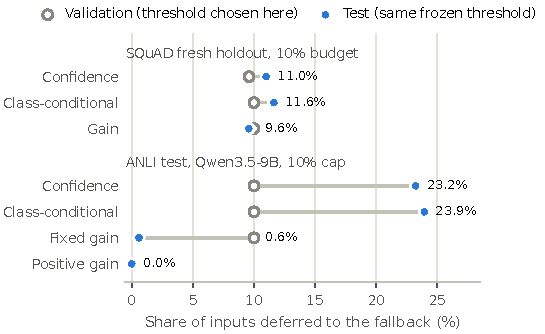
\includegraphics[width=\columnwidth]{figures/fig_budget_transfer.pdf}
\caption{Deferral rate on validation, where each threshold was chosen, and on test with the same frozen threshold, for Study~2 at its 10\% budget and Study~3 with the Qwen3.5-9B fallback. Appendix Table~\ref{tab:allrouting} gives both rates for all 17 settings.}
\label{fig:budget}
\end{figure}

Fixed thresholds also failed to hold the intended budget (Figure~\ref{fig:budget}). On the SQuAD holdout at the 10\% budget the realised rates stayed within 1.7 points of their validation values, and within 2.3 points across all three budgets (gain at 20\%: 20.0\% on validation, 17.7\% on test). On ANLI the confidence threshold deferred 23.2\% of test inputs against 10\% on validation, while the fixed-gain threshold deferred 0.6\%. StartLux's mean maximum probability fell from 0.882 on validation to 0.778 on the official test, so a threshold on confidence admits many more inputs, and the gain head scores the same inputs as less promising.

\subsection{RQ3: Serving}

\begin{figure*}[t]
\centering
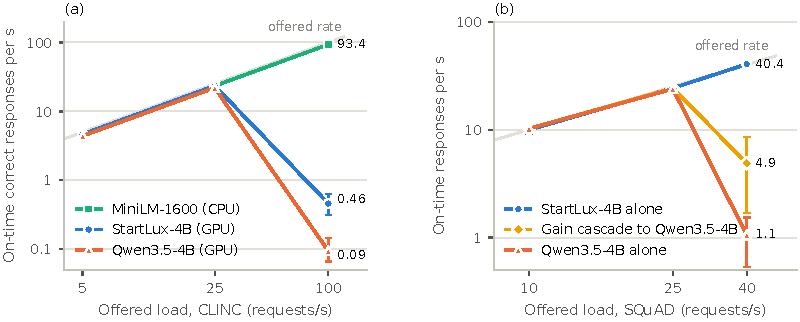
\includegraphics[width=\textwidth]{figures/fig_serving.pdf}
\caption{Open-loop serving with a 500\,ms SLO, log-log axes. (a) CLINC service study: on-time correct responses per second, median of five 180\,s rounds with min--max whiskers. (b) Study~2 on SQuAD: on-time responses per second, mean of three 30\,s rounds with min--max whiskers; the co-resident condition with Qwen idle matches StartLux alone and is omitted. Gray diagonals mark the offered rate.}
\label{fig:serving}
\end{figure*}

\begin{figure*}[t]
\centering
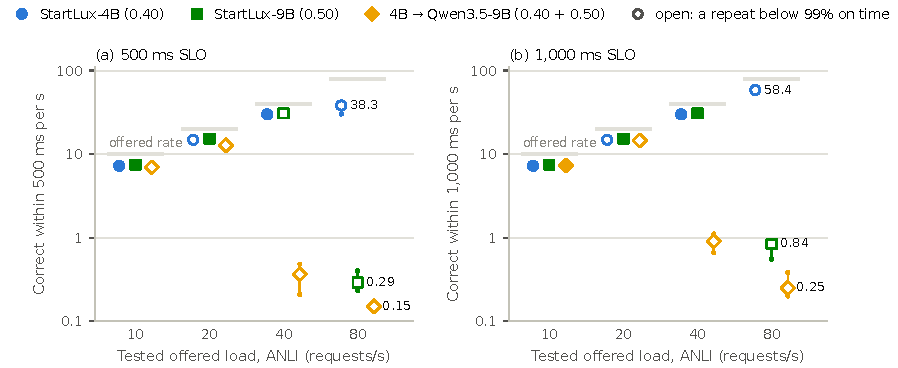
\includegraphics[width=\textwidth]{figures/fig_upgrade_serving.pdf}
\caption{ANLI 9B serving follow-up: correct answers per second at (a) a 500\,ms and (b) a 1,000\,ms SLO, counting the requests scheduled in the 120\,s arrival window that returned the correct label within their own SLO, divided by 120\,s; rejected and late requests stay in the offered base. Log y-axis. Each x-axis group is one tested rate, with the deployments offset inside it for legibility and a grey bar at the offered rate; no other rate was measured. Each marker is the median of three rounds and the whisker ends are the other two rounds; a marker is filled when every round answered at least 99\% of offers on time. GPU memory shares in parentheses. StartLux-4B at 20 requests/s keeps its round whose 78 late answers came from requests scheduled within a 3.6\,s span.}
\label{fig:upgrade}
\end{figure*}

\begin{table}[t]
\centering
\small
\setlength{\tabcolsep}{3pt}
\resizebox{\columnwidth}{!}{%
\begin{tabular}{lrrrr}
\toprule
Service & Rate & On-time corr./s & Done/s & p95 ms \\
\midrule
MiniLM-1600 (CPU) & 25 & 23.44 & 25.16 & 8.4 \\
StartLux-4B & 25 & 23.52 & 25.16 & 112.1 \\
Qwen3.5-4B & 25 & 22.01 & 25.16 & 344.2 \\
\midrule
MiniLM-1600 (CPU) & 100 & 93.43 & 100.29 & 15.2 \\
StartLux-4B & 100 & 0.46 & 64.71 & 1,041.1 \\
Qwen3.5-4B & 100 & 0.09 & 47.48 & 1,419.3 \\
\bottomrule
\end{tabular}
}
\caption{CLINC service study, medians of five rounds. Done/s counts all successful responses, on time or late. At 100 requests/s the client rejected 34.9\% of StartLux and 52.8\% of Qwen requests.}
\label{tab:serving}
\end{table}

In closed-loop serving at concurrency 8, direct StartLux processed 59.10 inputs/s on CLINC and 57.88 on SQuAD, against 32.71 and 30.76 for Qwen, and used 16.9--17.3 GPU-seconds per 1,000 decisions against 30.6--32.5. Adding the Qwen fallback to StartLux on SQuAD cut throughput to 44.21 inputs/s ($-23.6\%$) and raised the mean round p95 latency from 150.6 to 249.7\,ms, with both models resident on one GPU.

Open-loop load separates the deployments more sharply (Figure~\ref{fig:serving}). In Study~2 no condition rejected requests at 10 or 25 requests/s, and every round finished at least 91\% of its requests within the SLO; the lowest round (91.4\%) was StartLux alone at 10 requests/s, during a client dispatch stall of about two seconds. At 40 requests/s StartLux alone delivered 40.43 on-time responses per second, the same as with Qwen resident and idle, while the frozen gain cascade delivered 4.89 and Qwen alone 1.06. Keeping a second model resident cost nothing measurable at these loads; calling it did.

The service study extends the comparison to the CPU classifier (Table~\ref{tab:serving}). At 5 requests/s every request to every service finished within the SLO, and at 25 requests/s every request to MiniLM and StartLux did. Qwen finished 98.85\% of its 25 requests/s offers on time over the five rounds. One round had 12 rejections, 245 late responses and a p95 of 674.5\,ms, and the other four rounds had p95 between 342.9 and 348.7\,ms. At these loads on-time correct output tracked accuracy. At 100 requests/s the two GPU services saturated under our client and vLLM settings. StartLux still completed 64.7 requests/s and Qwen 47.5, and queueing pushed almost all of those completions past 500\,ms. MiniLM answered all 90,342 requests in the five rounds on time with p95 near 15\,ms. Its single inference thread used about 92 CPU-seconds per 180-second round (0.51 core-equivalents on average, on a node whose affinity allowed 16 logical CPUs) and about 200\,MiB of memory; StartLux ran at 96\% sampled GPU utilisation with a sampled memory peak of 18.9\,GiB. Label variability was also observed during repeated serving. Two CLINC inputs received more than one label from StartLux and eight from Qwen, while each MiniLM service's 117,451 responses matched its saved predictions exactly. Batch composition and numerical nondeterminism are candidate causes that this study did not separate.

The size control left open whether StartLux-9B's accuracy gain survives serving, so a follow-up measured it against the most accurate frozen Study~3 cascade (Figure~\ref{fig:upgrade}). Across its 36 cells, 131,935 of 162,801 offered requests were answered and the other 30,866 rejected by the client limit, with no model errors or timeouts. At 10 and 20 requests/s StartLux-9B returned the most correct answers within 500\,ms, 7.47 and 15.33 per second against 7.26 and 14.85 for StartLux-4B and 6.95 and 12.76 for the cascade. At 40 requests/s the cascade fell to 0.37 per second while StartLux-9B delivered 30.75 and StartLux-4B 29.96. StartLux-9B's weakest round there answered 98.87\% of offers on time, just under our 99\% rule, which StartLux-4B met in all three rounds. At 80 requests/s StartLux-4B had the highest correct goodput, 38.26 correct answers per second within 500\,ms and 58.41 within 1,000\,ms, against 0.29 and 0.84 for StartLux-9B and 0.15 and 0.25 for the cascade, whose requests the client rejected 56--57\% of the time; none of StartLux-4B's rounds met the 99\% rule at this rate, and its weakest answered 50.66\% of offers within 500\,ms. The rates passing the 99\% rule at 500\,ms were 10 and 40 requests/s for StartLux-4B, 10 and 20 for StartLux-9B and none for the cascade; at 1,000\,ms StartLux-9B also passed at 40 and the cascade at 10. StartLux-4B failed at 20 requests/s because one round returned 78 late answers for requests scheduled within 3.6\,s; the wait fell outside the recorded model-call time and its cause was not isolated. We kept that round, so the passing rates describe the tested points only. Live accuracy on answered requests stayed close to that of the saved predictions for the same requests (74.174\% against 74.124\% for StartLux-4B, 76.645\% against 76.640\% for StartLux-9B and 74.119\% against 74.342\% for the cascade; we ran no equivalence test), and the cascade deferred 23.3--24.7\% of answered requests against 23.9\% offline. Sampled GPU memory peaked at 17.7--19.5\,GiB for StartLux-4B, 22.0--22.7\,GiB for StartLux-9B and 39.7--40.4\,GiB for the cascade.

\section{Discussion}

\paragraph{When decision models replace generative calls.}
On these classification-shaped tasks StartLux-4B was more accurate and faster than the same-size generative model, and it adds probabilities that a gate can use. Where labelled data for a fixed intent set exists, a frozen encoder with a logistic head came within 0.33 points of it (559 versus 561 of 600, without an equivalence test) and stayed on time at a load that saturated both GPU services in our setup, with weaker OOS rejection that has to be checked for the target traffic. Where more accuracy is needed, the ANLI size control favours a larger decision model over the generative-fallback cascades we evaluated, and the serving follow-up points the same way for these checkpoints, this router and our serving settings. StartLux-9B's median correct goodput exceeded the frozen cascade's at every tested load and at both SLOs while it held a smaller memory share (0.50 against 0.90). StartLux-4B returned the most correct answers on time at 80 requests/s, though no round met the 99\% rule there, and it met that rule at 40 requests/s and 500\,ms where StartLux-9B missed it, so the choice between the two direct models depends on whether accuracy or headroom is the binding constraint.

\paragraph{Why deferral did not pay.}
Complementarity was present in every study. The matched-quota oracle sits 3.05 points above the StartLux cascade on SQuAD, and the ANLI fallback could rescue 289 inputs. The fallback was weaker on average, and the inputs it would rescue looked like the inputs it would harm to a router that sees confidence, predicted class and length. The positive-gain policy turned that into the safest available action, deferring nothing. Finding rescuable inputs would need richer routing features, such as text embeddings, together with confirmation on data no policy has seen. Serving adds its own price. In the follow-up, the class-conditional cascade, the most accurate one offline, sent about a quarter of its requests through a second model, returned fewer correct answers within 500\,ms than either direct model at every tested rate, and collapsed from 40 requests/s.

\paragraph{Operating points are distribution-specific.}
Both the risk target and the deferral budget moved with the confidence distribution of the test data, and prevalence alone changed measured risk on CLINC. A threshold tuned offline is a starting point that needs monitoring and recalibration on target traffic; finite-sample risk control \citep{angelopoulos2021ltt} and online budget enforcement are the natural next steps.

\section{Limitations}

We compare released checkpoints with fixed prompts and interfaces, so differences between systems mix architecture, training data and interface effects, and pretraining exposure to these public datasets is unknown. The CPU baselines and the StartLux-9B size control reuse test sets that earlier studies had already scored, and secondary results in Studies~2 and~3 are descriptive. Eight cells of the direct-accuracy matrix were not measured (Table~\ref{tab:direct}): Kev-4B on S2 and ANLI, and both 9B models on CLINC and the two SQuAD splits. The 4B-versus-9B comparisons therefore rest on ANLI alone, and Kev-4B enters only the CLINC and S1 comparisons. All serving numbers come from one GPU type with fixed client and vLLM settings (memory share 0.40 per model, except 0.50 for each 9B model in the 9B follow-up; StartLux front-end limit of 16 in-flight requests); capacities will move with these settings, and the offered rates bracket the saturation point without locating it. The CLINC service study spans two Slurm allocations with different physical L40S cards, and one of its fifteen paired groups crosses allocations; the 9B follow-up ran all 36 cells in a single further allocation on one card. The closed-loop timer excludes client queueing, which the open-loop SLO includes. The 9B follow-up compares three fixed deployments that differ in memory share as well as model, so it does not isolate the effect of model size, architecture or co-residency; its cascade router was chosen retrospectively, its accuracy reuses the ANLI test, and three rounds per rate describe serving variability without a significance test. We did not measure dollar cost, and the CPU baselines ran on a node that also held an idle GPU. SQuAD is reduced to answerability. Bootstrap intervals condition on frozen choices and carry no multiplicity correction.

\section{Conclusion}

For the fixed-label decisions studied here, a decision model can replace the generative call outright, and a supervised encoder can replace both when labels exist and load is high. A generative fallback earns its place only when a router can find the inputs it would fix and the deployment has capacity for its latency. With StartLux as the front model, the prespecified primary routers found no net gain on either holdout, and at the highest loads we tested the cascade missed the latency SLO. Deferral did help the weaker Kev front model. With the Qwen3.5-4B fallback on SQuAD, at least 99\% of cascade requests in every round met the SLO at 10 and 25 requests/s, while for the ANLI cascade with the 9B fallback no tested rate met the rule that every round answers at least 99\% of requests within 500\,ms. On ANLI, spending the extra GPU memory on a larger decision model returned more correct answers on time than spending it on a generative fallback, at every load we measured. Next steps are online budget control, routers with richer features confirmed on unseen data, and serving comparisons across memory budgets and hardware.

\section*{Team responsibilities}
Responsibilities for the final delivery are allocated as follows. Ju Zhang: experimental design, runtime and pipeline implementation, integration and final technical review. Weiyu Chen: statistical verification, interpretation and manuscript review. Yizhi Hu: reproducibility checks, the demo walkthrough and presentation materials.

\section*{Acknowledgments}
We thank our TA, Aman Upganlawar, whose feedback on 23 October 2026 shaped the data, comparison, ablation and metric choices (Appendix~A).

\bibliography{references}

\appendix

\section{TA Feedback}
\label{app:ta}

\begin{table}[h]
\centering
\small
\begin{tabular}{p{0.33\columnwidth}p{0.55\columnwidth}}
\toprule
Feedback (23 Oct 2026) & Where addressed \\
\midrule
State the data and how it is acquired & \S3, Table~\ref{tab:data}; SHA-pinned official sources and hashed splits \\
Specify the comparison methods & \S4: direct, always-generative, cascades, random and oracle routing, four routers \\
Include ablations & released vs.\ refitted temperature; random vs.\ confidence vs.\ oracle; class-conditional, gain and positive gain; 4B vs.\ 9B fallback; resident-idle vs.\ cascade; 400 vs.\ 1,600 labels; TF-IDF vs.\ MiniLM; 4B vs.\ 9B decision model, in accuracy and under serving load \\
Define the evaluation metrics & \S4: coverage and selective risk, accuracy, NLL/Brier/ECE, rescue and harm, latency, throughput, SLO goodput and correct goodput at 500 and 1,000\,ms \\
Newly released models may be used & Qwen3.5-9B and StartLux-9B added in Study~3 and the size control \\
A UI is optional & CPU Decision Lab provided as the demo (Appendix~C) \\
\bottomrule
\end{tabular}
\caption{TA feedback and where the report addresses it.}
\label{tab:ta}
\end{table}

\section{Additional Results}

Table~\ref{tab:allrouting} gives every routing policy evaluated on the two sealed holdouts. The Study~1 matched-quota comparison and probability quality follow in Tables~\ref{tab:oracle} and~\ref{tab:prob}.

\begin{table*}[t]
\centering
\small
\setlength{\tabcolsep}{4.5pt}
\begin{tabular}{llrrrrrr}
\toprule
 & & Val.\ defer & \multicolumn{2}{c}{Test defer} & & & Rescue / \\
\cmidrule(lr){4-5}
Setting & Policy & \% & $n$ & \% & Correct & Acc.\ \% & harm \\
\midrule
\multicolumn{8}{l}{\emph{Study~2: SQuAD S2 holdout ($n{=}4{,}000$), Qwen3.5-4B fallback; setting = validation call budget}} \\
5\% & Confidence & 4.3 & 198 & 4.950 & 3,690 & 92.250 & 55 / 36 \\
5\% & Class-conditional$^{s}$ & 4.5 & 260 & 6.500 & 3,716 & 92.900 & 92 / 47 \\
5\% & Gain & 5.0 & 194 & 4.850 & 3,669 & 91.725 & 0 / 2 \\
10\% & Confidence (reference) & 9.6 & 440 & 11.000 & 3,673 & 91.825 & 93 / 91 \\
10\% & Class-conditional & 10.0 & 465 & 11.625 & 3,669 & 91.725 & 105 / 107 \\
10\% & Gain$^{s}$ (primary) & 10.0 & 383 & 9.575 & 3,664 & 91.600 & 0 / 7 \\
20\% & Confidence & 19.8 & 848 & 21.200 & 3,604 & 90.100 & 109 / 176 \\
20\% & Class-conditional & 19.9 & 836 & 20.900 & 3,601 & 90.025 & 115 / 185 \\
20\% & Gain$^{s}$ & 20.0 & 709 & 17.725 & 3,662 & 91.550 & 0 / 9 \\
\midrule
\multicolumn{8}{l}{\emph{Separate reference: Study~1 gate replayed on S2; setting = 5\% selective-risk target, no call budget}} \\
5\% risk & Study~1 gate & 5.3 & 219 & 5.475 & 3,693 & 92.325 & 61 / 39 \\
\midrule
\multicolumn{8}{l}{\emph{Study~3: ANLI test ($n{=}3{,}200$), 10\% validation cap; setting = fallback}} \\
Qwen3.5-4B & Confidence & 10.0 & 743 & 23.219 & 2,229 & 69.656 & 98 / 243 \\
Qwen3.5-4B & Class-conditional & 10.0 & 766 & 23.938 & 2,273 & 71.031 & 94 / 195 \\
Qwen3.5-4B & Fixed gain & 10.0 & 29 & 0.906 & 2,374 & 74.188 & 0 / 0 \\
Qwen3.5-4B & Positive gain & 0.0 & 0 & 0.000 & 2,374 & 74.188 & 0 / 0 \\
Qwen3.5-9B & Confidence (reference) & 10.0 & 743 & 23.219 & 2,355 & 73.594 & 147 / 166 \\
Qwen3.5-9B & Class-conditional & 10.0 & 766 & 23.938 & 2,381 & 74.406 & 164 / 157 \\
Qwen3.5-9B & Fixed gain & 10.0 & 19 & 0.594 & 2,374 & 74.188 & 0 / 0 \\
Qwen3.5-9B & Positive gain (primary) & 0.0 & 0 & 0.000 & 2,374 & 74.188 & 0 / 0 \\
\bottomrule
\end{tabular}
\caption{Every routing policy evaluated on the two sealed holdouts, with a separate replay of the Study~1 gate. All rows use the StartLux-4B front model, whose direct accuracy is 91.775\% on S2 and 74.188\% on ANLI. Val.\ defer is the deferral rate on the validation set where each threshold was frozen (the 1,000 Study~1 SQuAD validation questions, which Study~2 reused, and 900 ANLI items). A budget or cap is an upper limit on that rate; a threshold defers whole groups of tied scores, so the rate can fall below it. The test columns apply the same frozen threshold. Rescue: front wrong and fallback right; harm: the reverse. (primary) and (reference) mark the two arms of each study's single prespecified primary comparison, as in Table~\ref{tab:routing}; every other row is descriptive, including class-conditional routing at 5\%. $^{s}$The candidate that validation selected at that budget, choosing between class-conditional and gain; only the 10\% selection was primary. The Study~1 gate keeps its Study~1 temperature and threshold, targets at most 5\% selective risk on validation, where it rejected 53 of the 1,000 questions, and has no call budget. Zeros are measured. Both positive-gain policies froze at zero deferrals, and fixed gain deferred 29 and 19 test items with no rescue or harm.}
\label{tab:allrouting}
\end{table*}

\begin{table}[h]
\centering
\small
\setlength{\tabcolsep}{3pt}
\resizebox{\columnwidth}{!}{%
\begin{tabular}{llrrrr}
\toprule
Task & Front & $k$ & Random & Gate & Oracle \\
\midrule
CLINC & Kev (rel.) & 210 & 81.18 & 86.17 & 91.00 \\
CLINC & Kev (refit) & 215 & 81.26 & 85.67 & 91.00 \\
CLINC & StartLux & 1 & 93.49 & 93.50 & 93.67 \\
SQuAD & Kev & 1,292 & 84.35 & 85.85 & 90.85 \\
SQuAD & StartLux & 125 & 90.92 & 91.50 & 94.55 \\
\bottomrule
\end{tabular}
}
\caption{Study~1 cascade accuracy (\%) with $k$ deferrals to Qwen3.5-4B: random routing (expectation), the frozen confidence gate, and the hindsight oracle.}
\label{tab:oracle}
\end{table}

\begin{table}[h]
\centering
\small
\setlength{\tabcolsep}{2.5pt}
\resizebox{\columnwidth}{!}{%
\begin{tabular}{llrrrr}
\toprule
Task & Model & $T$ & NLL & Brier & ECE \\
\midrule
CLINC & Kev & 0.831 & .619$\to$.627 & .305$\to$.313 & .058$\to$.056 \\
CLINC & StartLux & 0.831 & .246$\to$.260 & .104$\to$.105 & .027$\to$.025 \\
SQuAD & Kev & 1.295 & .432$\to$.422 & .274$\to$.271 & .042$\to$.021 \\
SQuAD & StartLux & 0.958 & .216$\to$.217 & .128$\to$.128 & .013$\to$.016 \\
\bottomrule
\end{tabular}
}
\caption{Probability quality on Study~1 test sets, released $\to$ refitted temperature (lower is better).}
\label{tab:prob}
\end{table}

\section{Reproducibility}

Code, protocols, reports and audit receipts are in the project repository:
\begin{center}\small\url{https://github.com/jzdscience/e6998_llm_genai_decision_study}\end{center}
Raw result bundles and model weights stay outside Git and are indexed by SHA-256 in \nolinkurl{records/BUNDLE_INDEX.json}. Table~\ref{tab:bundles} lists the accepted bundles. The figures in this paper are regenerated from tracked files with \nolinkurl{paper/figures/make_figures.py}. \nolinkurl{reports/followups-2026-11-06/audit/README.md} reruns the audits of the service study and the size control, and \nolinkurl{reports/upgrade-9b-serving-2026-11-09/audit/README.md} reruns the integrity and raw-metric audits of the 9B serving follow-up from its original archives. The CPU-only Decision Lab (\nolinkurl{scripts/run_lab.sh}) replays recorded cases from Studies~1--3 and shows the measured follow-ups without a GPU. \nolinkurl{scripts/reproduce_cpu.sh} runs the CPU test suite, the Lab evidence check, the follow-up audit reruns, the report and figure regeneration and the paper build in a few minutes. For the 11/6 follow-ups it compares ten audit receipts byte for byte and two after removing a recorded run-context field. For the 9B follow-up it compares the six audit receipts, the Lab follow-up evidence and the report tables byte for byte. It compares the figures byte for byte when the Matplotlib version pinned in \nolinkurl{paper/requirements-figures.txt} is installed, and \texttt{-{}-strict} turns every skipped step, including a missing raw input, into a failure.

\begin{table}[h]
\centering
\scriptsize
\setlength{\tabcolsep}{2.5pt}
\begin{tabular}{lll}
\toprule
Study & Bundle SHA-256 (prefix) & Source \\
\midrule
Study 1 predictions & \texttt{be748917f2f2184e} & frozen v1 \\
Study 1 closed-loop serving & \texttt{72138989815c0422} & frozen v1 \\
Study 2 & \texttt{f340f4b159cb21a0} & v2 release \\
Study 3 & \texttt{a8d0dc672d83c3ed} & v3 release \\
TF-IDF-400 baseline & \texttt{7fcd28785a06bf23} & \texttt{797aff1} \\
TF-IDF-1600, MiniLM & \texttt{7f00178c7bd1d86e} & \texttt{1b70899} \\
Service study & \texttt{d212c130c707a30f} & \texttt{8b5370d} \\
StartLux-9B size control & \texttt{f427f7762bac745d} & \texttt{8b5370d} \\
9B serving preflight & \texttt{8adafb29ff4501e5} & \texttt{7c81947} \\
9B serving follow-up & \texttt{9baeca3eb7f84a86} & \texttt{7c81947} \\
\bottomrule
\end{tabular}
\caption{Accepted result bundles.}
\label{tab:bundles}
\end{table}

Pinned model revisions: Kev-4B \texttt{139fdd94}, StartLux-4B \texttt{416088f7}, StartLux-9B \texttt{18a17f73}, Qwen3.5-4B \texttt{851bf6e8}, Qwen3.5-9B \texttt{c2022362}, all-MiniLM-L6-v2 \texttt{1110a243}.

\end{document}
